
\documentclass{article}

\usepackage[margin=0.5in]{geometry}
\usepackage{multicol}
\usepackage{tkz-euclide}
\usetikzlibrary{decorations.markings,arrows}
\tikzset{
    arrowMe/.style={
        postaction=decorate,
        decoration={
            markings,
            mark=at position .5 with {\arrow[thick]{#1}}
        }
    }
}

\title{Problem-Solving Set A}
\author{}
\date{}

\begin{document}
\maketitle
\noindent Problems should be solved without a calculator unless otherwise specified.
Remember to explain how you solved a problem.
\begin{multicols*}{2}
    \begin{enumerate}
        \item Five cards are lying on a table as shown.
            \begin{center}
                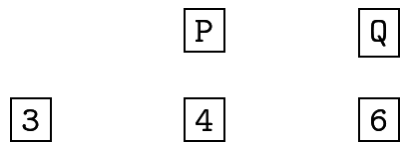
\includegraphics[scale=0.25]{5-2_cards.png}
            \end{center}
            Each card has a letter on one side and a whole number on the other side.
            Janes said, ``If a vowel is on one side of any card, then an even number is on the other side.''
            Mary showed Jane was wrong by turning over one card.
            Which card did Mary turn over?
            \vspace{3cm}
        \item In a magic triangle, each of the six whole numbers $10$ - $15$ is placed in one of the circles so that the sum, $S$ of the three numbers on each side of the triangle is the same.
            What is the the largest possible for $S$?
            \begin{center}
                \begin{tikzpicture}[scale=0.75]
                    \tkzDefPoint(0,0){A}
                    \tkzDefPoint(60:4){B}
                    \tkzDefPoint(4,0){C}
                    \tkzDrawPolygon(A,B,C)

                    \foreach \initpoint\finpoint\name in {A/B/D, C/B/E, C/A/F}
                    {
                        \tkzDefMidPoint(\initpoint,\finpoint)
                        \tkzGetPoint{\name}
                    }

                    \foreach \point in {A, B, C, D, E, F}
                    {
                        \tkzDrawCircle[R,fill=white](\point,0.25cm)
                    }
                \end{tikzpicture}
            \end{center}
            \vspace{3cm}
        \item Alan, Beth, Carlos, and Diana were discussing their possible grades in mathematics class this grading period.
            Alan said, ``If I get an A, then Beth will get an A.''
            Beth said, ``If I get an A, then Carlos will get an A.''
            Carlos said, ``If I get an A, then Diana will get an A.''
            All of these statements were true, but only two of the students received an A.
            Which two received A's?
            \vspace{3cm}
        \item Let $o$ be an odd whole number and let $n$ be any whole number.
            Which of the following statements about the whole number $(o^2 + no)$ is always true?
            \begin{itemize}
                \item It is always odd.
                \item It is always even.
                \item It is even only if $n$ is even.
                \item It is odd only if $n$ is odd.
                \item It is odd only if $n$ is even.
            \end{itemize}
            \vspace{3cm}
        \item Using only the paths and the directions shown, how many different routes are there from $M$ to $N$.
            \begin{center}
                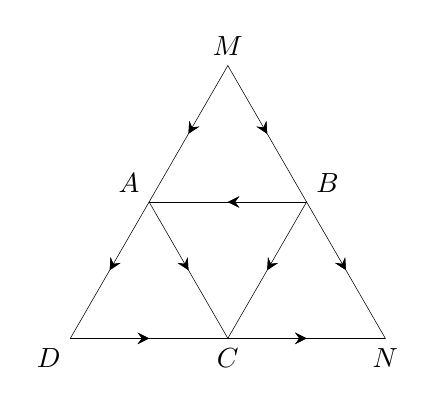
\begin{tikzpicture}
                    \tkzDefPoint(0,0){D}
                    \tkzDefPoint(60:4){M}
                    \tkzDefPoint(4,0){N}

                    \foreach \initpoint\finpoint\name in {D/M/A, M/N/B, D/N/C}
                    {
                        \tkzDefMidPoint(\initpoint,\finpoint)
                        \tkzGetPoint{\name}
                    }

                    \tkzLabelPoint[below left](D){$D$}
                    \tkzLabelPoint[above](M){$M$}
                    \tkzLabelPoint(N){$N$}
                    \tkzLabelPoint[above left](A){$A$}
                    \tkzLabelPoint[above right](B){$B$}
                    \tkzLabelPoint[below](C){$C$}

                    \tkzDrawSegments[arrowMe=stealth](M,A M,B B,A A,C B,C A,D D,C C,N B,N)
                \end{tikzpicture}
            \end{center}
            \vspace{3cm}
    \end{enumerate}
\end{multicols*}
\end{document}